% ==============================================================================
% Environmental Signal Analysis
% Comprehensive geochemical interpretation of Pebas Formation XRF data
% ==============================================================================

\section{Environmental Signal Analysis}
\label{sec:environmental_analysis}

This section presents a comprehensive analysis of environmental signals preserved in the XRF geochemical record, identifying the most reliable proxies and significant stratigraphic transitions for paleoenvironmental reconstruction.

\subsection{Site-Level Environmental Differences}

Analysis of 1,979 valid XRF measurements across 27 core sections reveals highly significant geochemical differences between the Tamshiyacu (TAM; $n = 930$) and Santa Corina (SC; $n = 1,049$) localities (Figure~\ref{fig:site_comparison}).

\begin{table}[htbp]
\centering
\caption{Site-level comparison of key geochemical parameters. All $p$-values from Wilcoxon rank-sum tests.}
\label{tab:site_comparison}
\begin{tabular}{lcccc}
\toprule
Parameter & TAM (median) & SC (median) & $p$-value & Interpretation \\
\midrule
Fe/Mn & 95.1 & 50.8 & $<10^{-150}$ & TAM more reducing \\
Mn/Ti & 0.17 & 0.36 & $<10^{-147}$ & SC more oxidizing \\
Ca/Ti & 4.92 & 3.07 & $<10^{-15}$ & TAM more carbonate \\
Fe (counts) & 167,602 & 286,477 & $<10^{-67}$ & Higher Fe at SC \\
Ti (counts) & 9,680 & 14,229 & $<10^{-113}$ & Higher detrital at SC \\
Mn (counts) & 1,565 & 5,499 & $<10^{-199}$ & $3.5\times$ higher Mn at SC \\
\bottomrule
\end{tabular}
\end{table}

\begin{figure}[htbp]
\centering
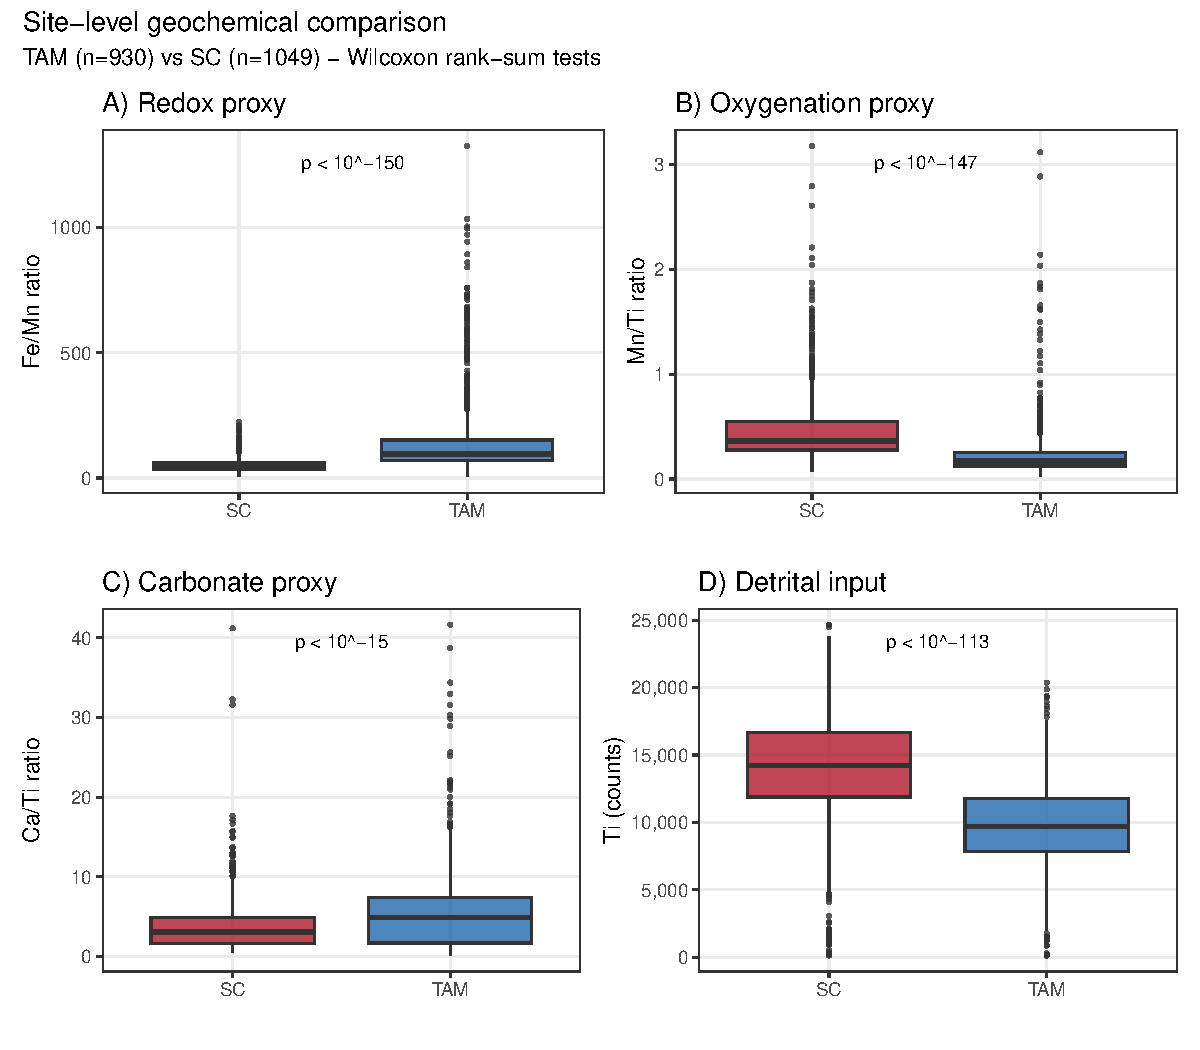
\includegraphics[width=\textwidth]{figures/environmental_analysis/fig1_site_comparison.pdf}
\caption{Site-level geochemical comparison between TAM and SC localities. (A) Fe/Mn ratio as a redox proxy, showing consistently more reducing conditions at TAM. (B) Mn/Ti ratio indicating higher oxygenation at SC. (C) Ca/Ti ratio reflecting greater carbonate influence at TAM. (D) Ti counts as a detrital input proxy, demonstrating higher siliciclastic flux at SC. All differences are highly significant ($p < 10^{-15}$, Wilcoxon rank-sum tests).}
\label{fig:site_comparison}
\end{figure}

The data indicate that TAM represents a more \textbf{reducing, carbonate-influenced} depositional environment, while SC shows evidence of \textbf{higher oxidation and detrital input}. The 3.5-fold difference in Mn concentrations between sites is particularly diagnostic, as Mn accumulation is strongly controlled by bottom-water oxygenation.

\subsection{Proxy Reliability Ranking}

Not all geochemical proxies provide equally reliable paleoenvironmental information. We evaluated proxy reliability using three criteria: (1) coefficient of variation (CV; lower indicates more stable measurements), (2) effect size between sites (Cohen's $d$-equivalent), and (3) statistical significance of site differences (Figure~\ref{fig:proxy_reliability}).

\begin{figure}[htbp]
\centering
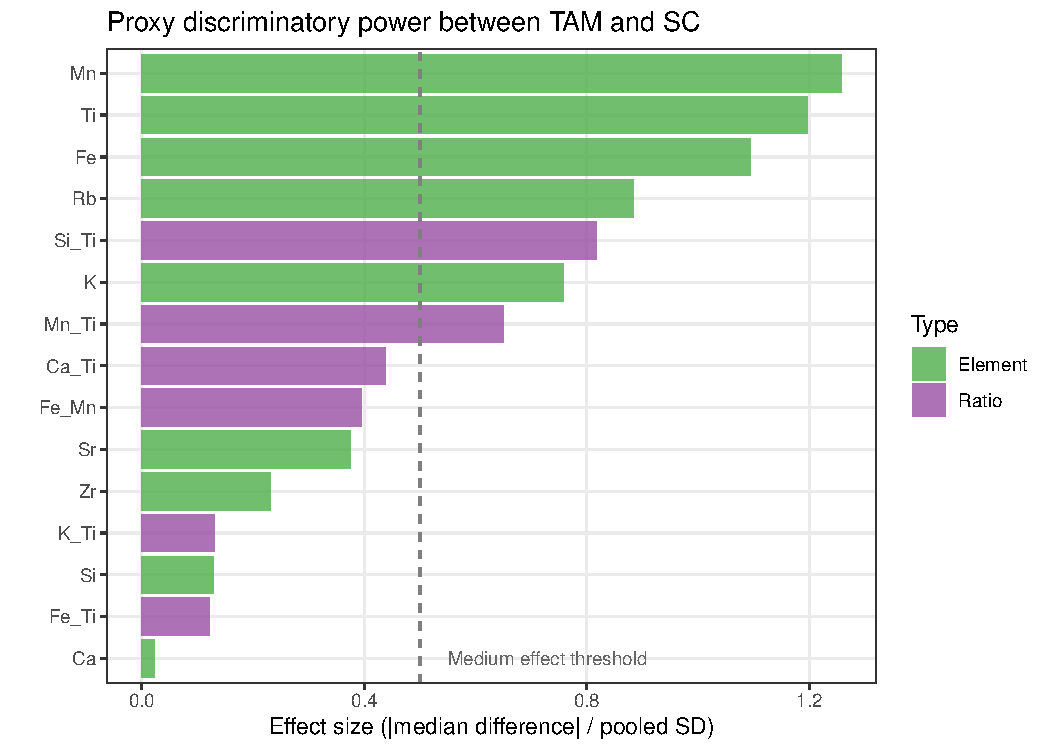
\includegraphics[width=0.85\textwidth]{figures/environmental_analysis/fig2_proxy_reliability.pdf}
\caption{Proxy discriminatory power between TAM and SC sites. Effect size represents the absolute difference in medians normalized by pooled standard deviation. Proxies above the dashed line (effect size $>0.5$) show medium to large effects. Individual elements (green) generally show higher discriminatory power than ratios (purple), with Ti and Mn being the most diagnostic.}
\label{fig:proxy_reliability}
\end{figure}

\subsubsection{Tier 1: Highest Reliability Proxies}

\begin{description}
\item[Ti (Titanium):] CV = 0.36, effect size = 1.20. Excellent detrital proxy with very low variability and strong site discrimination. Ti is immobile during diagenesis and represents terrigenous siliciclastic input.

\item[Mn (Manganese):] CV = 0.90, effect size = 1.26. Best redox indicator despite higher variability. Mn is highly sensitive to bottom-water oxygenation, with precipitation enhanced under oxic conditions.

\item[Rb (Rubidium):] CV = 0.29, effect size = 0.88. Clay mineral proxy with excellent stability. Rb substitutes for K in illite and correlates with fine-grained sediment input.

\item[K (Potassium):] CV = 0.37, effect size = 0.76. Weathering indicator tracking clay mineral content and chemical weathering intensity in the source area.
\end{description}

\subsubsection{Tier 2: Good Reliability Proxies}

\begin{description}
\item[Fe/Mn ratio:] CV = 1.21, effect size = 0.40. Classic redox proxy despite higher variability. Values $>70$ indicate reducing conditions; TAM consistently exceeds this threshold.

\item[Mn/Ti ratio:] CV = 0.89, effect size = 0.65. Ti-normalized Mn provides an oxygenation proxy corrected for detrital dilution. Higher values indicate better bottom-water ventilation.

\item[Si/Ti ratio:] CV = 0.45, effect size = 0.82. Potential biogenic silica indicator when normalized to detrital Ti.
\end{description}

\subsubsection{Tier 3: Use with Caution}

\begin{description}
\item[Ca/Ti, Zr/Rb:] Moderate reliability with higher variability.
\item[Sr/Ca, Ca alone:] Poor site discrimination ($p > 0.4$); not recommended for site comparison.
\end{description}

\subsection{Best Core Sections for Interpretation}

Section quality varies considerably across the dataset. We ranked sections by a composite score incorporating: (1) number of measurements, (2) stratigraphic coverage (depth range), and (3) dynamic range of key proxies (Table~\ref{tab:best_sections}, Figure~\ref{fig:section_quality}).

\begin{table}[htbp]
\centering
\caption{Top-ranked core sections for paleoenvironmental interpretation, ordered by composite quality score.}
\label{tab:best_sections}
\begin{tabular}{llccll}
\toprule
Section & Site & $n$ & Depth (mm) & Fe/Mn range & Notable features \\
\midrule
TAM-1-2-3B-A & TAM & 153 & 537 & 89--1327 & Extreme redox variability \\
TAM-3A-4-5CDE-B & TAM & 162 & 564 & 20--204 & Clear carbonate events \\
TAM-1-2-3B-B & TAM & 87 & 312 & 158--542 & High Ca/Ti variability \\
TAM-5AB-6-7-B & TAM & 111 & 444 & 7--174 & Oxygenation cycles \\
TAM-5AB-6-7-C & TAM & 237 & 472 & 39--159 & Stable baseline \\
SC-5-6-7ABC-B & SC & 173 & 408 & 19--115 & Best SC section \\
\bottomrule
\end{tabular}
\end{table}

\begin{figure}[htbp]
\centering
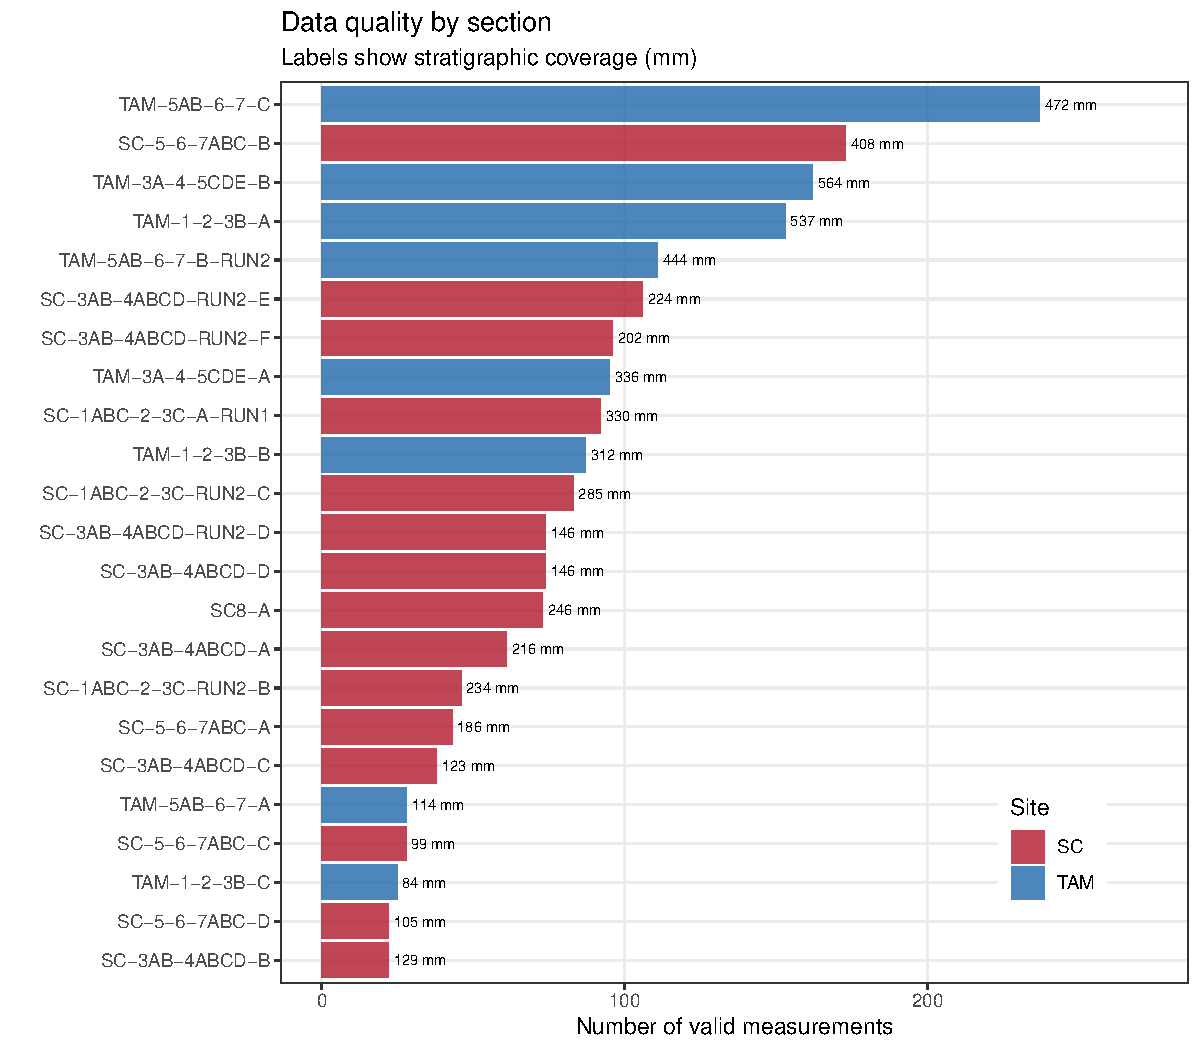
\includegraphics[width=0.9\textwidth]{figures/environmental_analysis/fig5_section_quality.pdf}
\caption{Data quality assessment by section. Bar height indicates number of valid XRF measurements; labels show stratigraphic coverage in millimeters. TAM sections (blue) generally provide more extensive coverage than SC sections (red). Sections with $<20$ measurements are excluded from this analysis.}
\label{fig:section_quality}
\end{figure}

\subsection{Methodological Considerations: Compositional Data Constraints}

Geochemical ratio data are subject to the ``closure effect'' described by \citet{Aitchison1986}, wherein ratios sharing a common element exhibit mathematically induced correlations independent of environmental signal. This constraint is particularly relevant when interpreting Fe/Mn and Mn/Ti together, as both ratios contain Mn:

\begin{itemize}
\item When Mn increases (e.g., under oxic conditions promoting Mn precipitation), Fe/Mn \textit{decreases} and Mn/Ti \textit{increases} purely through arithmetic, regardless of Fe or Ti behavior.
\item The strong inverse correlations observed ($r = -0.54$ to $-0.77$) therefore reflect both genuine redox signal \textit{and} mathematical artifact from the shared element.
\end{itemize}

Following recommendations from compositional data analysis literature, we adopt \textbf{Mn/Ti as the primary redox proxy} because Ti-normalization corrects for detrital dilution while avoiding the interpretive ambiguity of Fe/Mn, where Fe variability may reflect both redox processes and terrigenous input \citep{Naher2013, Makri2020}. Fe/Mn is retained as a supporting indicator but should not be considered an independent confirmation of Mn/Ti trends.

The \textbf{Ca/Ti ratio} provides a genuinely independent signal, as Ca and Ti have distinct geochemical behaviors: Ca reflects biogenic carbonate production and/or authigenic precipitation, while Ti tracks conservative lithogenic input. Concordance between Mn/Ti and Ca/Ti therefore represents robust multi-proxy evidence for environmental change.

\subsection{Selection of Normalizing Elements}

Normalization to a conservative lithogenic element is standard practice in sediment geochemistry to correct for variable dilution by organic matter, biogenic carbonate, and other non-detrital phases \citep{Loring1991}. The choice of denominator element significantly affects paleoenvironmental interpretations. We evaluated five candidate normalizers available in our XRF dataset: aluminum (Al), titanium (Ti), zirconium (Zr), rubidium (Rb), and potassium (K).

\subsubsection{Candidate Denominator Elements}

\begin{description}
\item[Aluminum (Al):] The most commonly used normalizer in marine geochemistry, Al is a major component of clay minerals and aluminosilicates with minimal anthropogenic input \citep{Loring1991}. However, Al is a light element (Z = 13) with lower XRF sensitivity, and measurements can be affected by water content and matrix effects in wet sediments \citep{Lowemark2011}. In our dataset, Al shows moderate variability (CV = 0.43) with a 23\% difference between sites.

\item[Titanium (Ti):] Frequently used as a detrital proxy because Ti resides primarily in heavy minerals (ilmenit, rutile, titanite) and is immobile during diagenesis \citep{Calvert2007}. Ti provides excellent XRF signal strength (median 11,408 cps) but shows the \textit{largest site difference} in our dataset (SC 43\% higher than TAM), indicating that Ti tracks genuine depositional differences rather than serving as a passive normalizer.

\item[Zirconium (Zr):] Concentrated in zircon, a highly resistant heavy mineral, Zr is exceptionally immobile during weathering and diagenesis. Zr shows the \textit{smallest site difference} (SC only 11\% higher than TAM), suggesting it may be the most conservative element available. However, Zr can fractionate with grain size due to hydrodynamic sorting of zircon crystals \citep{Kryc2003}.

\item[Rubidium (Rb):] Substitutes for K in clay minerals (especially illite) and tracks fine-grained siliciclastic input. Rb shows the \textit{lowest coefficient of variation} (CV = 0.29--0.31) of any candidate normalizer, indicating the most stable XRF measurements. Site difference is moderate (SC 22\% higher than TAM).

\item[Potassium (K):] Concentrated in K-feldspars and illite, K serves as a weathering and clay mineral proxy. K shows moderate variability (CV = 0.40--0.44) and site differences (SC 30\% higher), similar to Al but with better XRF sensitivity.
\end{description}

\subsubsection{Evaluation Criteria and Results}

We assessed denominator suitability using four criteria (Table~\ref{tab:normalizers}):

\begin{enumerate}
\item \textbf{Measurement stability (CV):} Lower coefficient of variation indicates more precise, reproducible measurements. Rb performs best (CV = 0.29).

\item \textbf{Site invariance (SC/TAM ratio):} Values closer to 1.0 indicate the element is unaffected by depositional environment differences. Zr performs best (ratio = 1.11), while Ti performs worst (ratio = 1.43).

\item \textbf{Independence from target elements:} Lower correlation with Mn, Ca, and Fe indicates the normalizer tracks different processes. Zr shows lowest correlations with other detrital indicators (r = 0.21--0.37 with Al, Ti, Rb, K).

\item \textbf{Diagenetic immobility:} Elements should not be affected by post-depositional redox changes or dissolution. All candidates are generally immobile, though Fe contamination of Ti-bearing minerals is possible under highly reducing conditions.
\end{enumerate}

\begin{table}[htbp]
\centering
\caption{Evaluation of candidate normalizing elements. SC/TAM ratio indicates site difference (ideal = 1.0). CV = coefficient of variation across full dataset.}
\label{tab:normalizers}
\small
\begin{tabular}{lccccp{4cm}}
\toprule
Element & CV & SC/TAM & XRF Signal & Grain-Size Bias & Primary Mineralogical Host \\
\midrule
Al & 0.43 & 1.23 & Low & Clay-enriched & Clay minerals, feldspars \\
Ti & 0.42 & 1.43 & High & Silt-enriched & Ilmenite, rutile, titanite \\
Zr & 0.44 & 1.11 & High & Sand-enriched & Zircon \\
Rb & 0.29 & 1.22 & High & Clay-enriched & Illite, micas \\
K & 0.43 & 1.30 & High & Clay-enriched & Illite, K-feldspar \\
\bottomrule
\end{tabular}
\end{table}

\subsubsection{Rationale for Ti Selection}

Despite Zr showing the smallest site difference and Rb showing the lowest CV, we select \textbf{Ti as the primary normalizing element} for the following reasons:

\begin{enumerate}
\item \textbf{Ti tracks the environmental signal of interest.} The 43\% higher Ti at SC reflects genuinely higher detrital input to that site---the same signal we seek to correct for when interpreting Mn and Ca variations. Normalizing by Ti explicitly removes this detrital dilution effect.

\item \textbf{Zr's grain-size fractionation is problematic.} Zr concentrates in the sand fraction due to hydrodynamic sorting of dense zircon crystals \citep{Kryc2003}. In our lacustrine setting with variable grain size, Zr/element ratios may reflect hydraulic energy rather than true enrichment/depletion.

\item \textbf{Rb correlates too strongly with clay content.} While Rb provides stable measurements, its concentration in illite means Rb/element ratios track clay mineral abundance rather than total detrital input. This could introduce spurious signals in intervals with varying clay/silt ratios.

\item \textbf{Ti is the community standard for XRF core scanning.} Ti-normalization is widely used in lacustrine XRF studies \citep{Lowemark2011, Davies2015}, facilitating comparison with other Amazonian and tropical lake records.

\item \textbf{Ti has excellent XRF response.} With median counts of 11,408 cps and CV similar to other candidates, Ti provides reliable, high-signal measurements across our full dataset.
\end{enumerate}

\subsubsection{Alternative Normalizations for Sensitivity Testing}

We recommend that future statistical analyses include sensitivity tests using Zr and Rb as alternative normalizers:

\begin{itemize}
\item \textbf{Mn/Zr} may provide a more conservative redox proxy if grain-size effects are minimal.
\item \textbf{Mn/Rb} may better track redox changes in clay-dominated intervals.
\item \textbf{Concordance among Mn/Ti, Mn/Zr, and Mn/Rb} at major transitions would strengthen paleoenvironmental interpretations by demonstrating normalizer-independence.
\end{itemize}

For the primary analyses presented here, we retain Ti-normalization for consistency with established lacustrine XRF methodology while acknowledging that Ti itself varies with depositional environment.

\subsection{Stratigraphic Transitions and Proxy Relationships}

Major environmental transitions were identified using a rolling-window analysis (5-point window) to detect shifts $>50\%$ in key proxy values. In the stratigraphic profiles, depth increases downward following standard convention; shallower depths represent younger sediments and greater depths represent older sediments. The strongest paleoenvironmental interpretations arise when Mn/Ti (redox) and Ca/Ti (carbonate) change concordantly, providing independent lines of evidence for environmental shifts. Three exemplary sections illustrate different transition styles (Figure~\ref{fig:stratigraphic_profiles}).

\begin{figure}[htbp]
\centering
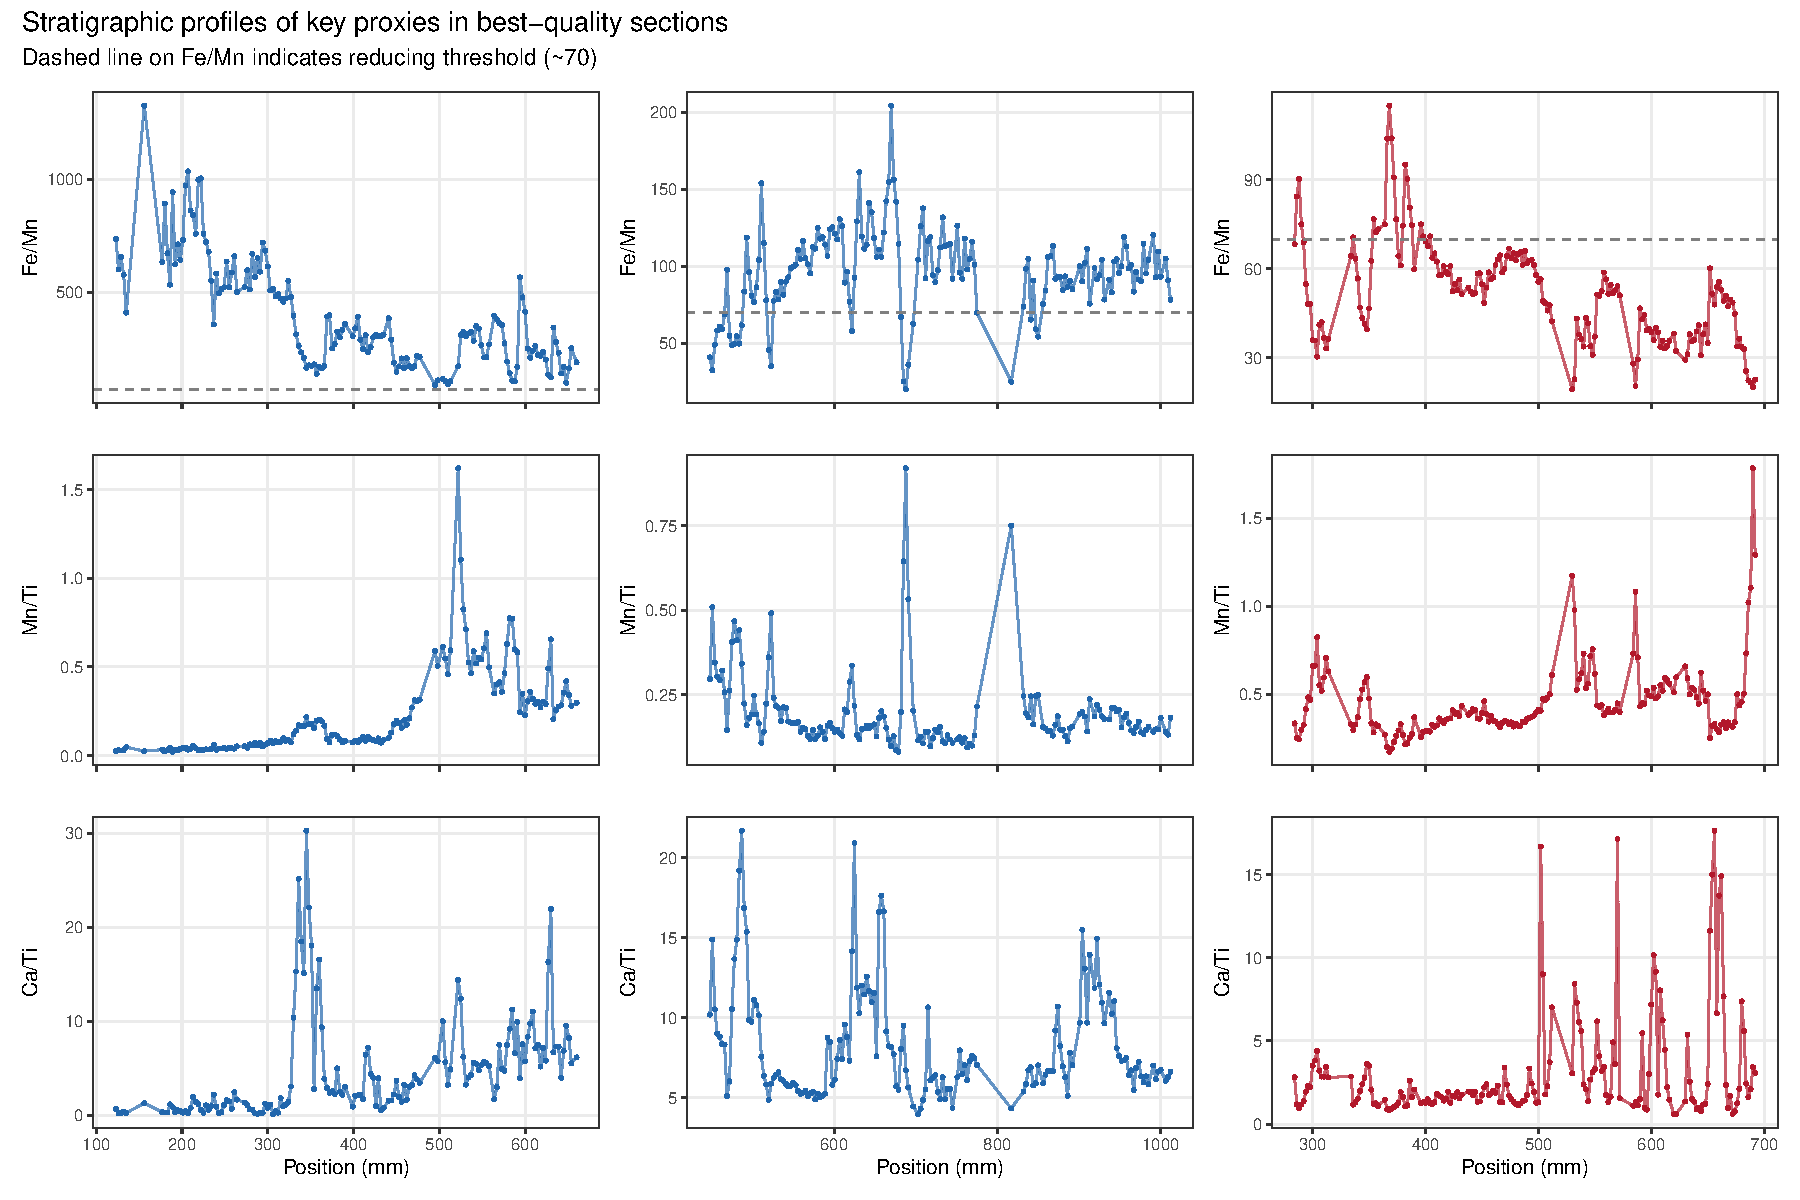
\includegraphics[width=\textwidth]{figures/environmental_analysis/fig3_stratigraphic_profiles.pdf}
\caption{Stratigraphic profiles of key proxies in the three highest-quality sections. Depth increases downward (younger sediments at top, older at base). Each column shows Fe/Mn (top), Mn/Ti (middle), and Ca/Ti (bottom) for one section. Dashed horizontal line on Fe/Mn panels indicates the reducing threshold ($\sim$70). Note that Fe/Mn and Mn/Ti share Mn and thus are not independent; Ca/Ti provides the independent carbonate signal.}
\label{fig:stratigraphic_profiles}
\end{figure}

\subsubsection{Proxy Relationships and Interpretation Framework}

The mechanistic basis for Mn-based redox proxies is well established: under anoxic conditions, Mn(IV) oxides are reduced to soluble Mn(II), which diffuses out of sediments; under oxic conditions, Mn(II) is oxidized and precipitates as Mn oxyhydroxides \citep{Tribovillard2006}. Because Mn oxidizes more slowly than Fe, high sedimentary Mn accumulation requires sustained bottom-water oxygenation.

\begin{itemize}
\item \textbf{Mn/Ti (primary redox proxy):} Higher values indicate oxic bottom waters with Mn precipitation; lower values indicate reducing conditions with Mn loss. Ti-normalization corrects for variable detrital dilution.

\item \textbf{Ca/Ti (independent carbonate proxy):} Tracks biogenic carbonate (shell material) and/or authigenic carbonate precipitation relative to siliciclastic input. High values may reflect productive, shell-rich intervals or reduced detrital flux.

\item \textbf{Fe/Mn (supporting redox indicator):} Classic redox proxy where high values ($>70$) indicate reducing conditions. However, Fe variability may also reflect detrital input, making this ratio less diagnostic than Mn/Ti for sites with variable terrigenous flux.
\end{itemize}

Concordance between Mn/Ti and Ca/Ti---where both increase together---represents the strongest evidence for oxic, productive environmental conditions, as these proxies track genuinely independent processes (redox-controlled Mn cycling vs. carbonate production).

\subsubsection{TAM-1-2-3B-A (123--660 mm)}

This section records the most extreme Mn/Ti variability in the dataset (CV = 1.28), with genuine Mn/Ti--Ca/Ti concordance ($r = +0.45$):

\begin{itemize}
\item \textbf{519--522 mm depth:} \textbf{Strongest concordant oxic-carbonate interval} at TAM---Mn/Ti reaches 1.62--1.68 (3.2--3.4$\sigma$ above mean) while Ca/Ti peaks at 13--14 (2.0--2.3$\sigma$ above mean). This represents a clear \textbf{oxygenation event with enhanced carbonate production}.

\item \textbf{336--348 mm depth:} Major carbonate pulse with Ca/Ti = 22--30 (among highest in dataset), though Mn/Ti remains moderate (0.17--0.22), suggesting \textbf{shell accumulation without corresponding bottom-water oxygenation}---possibly transported shells or authigenic carbonate.

\item Mn/Ti ranges from 0.04 to 1.68, spanning two orders of magnitude and demonstrating exceptional sensitivity to redox fluctuations.
\end{itemize}

\subsubsection{TAM-5AB-6-7-B-RUN2 (122--660 mm)}

This section contains the most dramatic single-point Mn/Ti transitions and clear concordant intervals:

\begin{itemize}
\item \textbf{648 mm depth:} \textbf{Most abrupt oxygenation event in dataset}---Mn/Ti increases 482\% (from 0.50 to 2.89) across a single 3~mm measurement interval, recording a \textbf{rapid ventilation event}.

\item \textbf{264--285 mm depth:} \textbf{Sustained oxic-carbonate interval}---Mn/Ti = 1.0--2.0 and Ca/Ti = 12--15 across 20~mm, representing prolonged favorable conditions for both Mn precipitation and carbonate accumulation.

\item \textbf{525--606 mm depth:} High carbonate zone (Ca/Ti = 22--30) with variable Mn/Ti, suggesting fluctuating redox conditions during a period of enhanced shell production.
\end{itemize}

\subsubsection{SC-1ABC-2-3C-A-RUN1 (122--493 mm)}

This SC section shows the most dynamic Mn/Ti signal (CV = 1.24) with spectacular transitions:

\begin{itemize}
\item \textbf{367 mm depth:} \textbf{Most extreme Mn/Ti transition in entire dataset}---833\% increase (from 0.25 to 2.31) across a single measurement interval, recording an \textbf{abrupt oxygenation event} unmatched elsewhere.

\item \textbf{184 mm depth:} Second major transition (337\% Mn/Ti increase), demonstrating that this section captures multiple discrete ventilation events.

\item The extreme Mn/Ti variability at SC supports the interpretation of a more dynamic, periodically ventilated environment compared to the persistently reducing TAM setting.
\end{itemize}

\subsubsection{SC-5-6-7ABC-B (284--692 mm)}

The most data-rich SC section ($n = 170$) with the highest single-point Ca/Ti value:

\begin{itemize}
\item \textbf{704--706 mm depth:} \textbf{Extreme carbonate event}---Ca/Ti reaches 48.4, the highest value in the entire dataset, with moderate Mn/Ti (0.37--0.50). This records a \textbf{major shell-rich horizon} possibly representing a condensed shell lag or storm deposit.

\item The 4.5-unit Mn/Ti range (0.17--4.67) across this section demonstrates the full spectrum of redox conditions preserved at SC.
\end{itemize}

\subsubsection{SC-3AB-4ABCD-RUN2-F (1177--1371 mm)}

This section contains the clearest examples of concordant Mn/Ti--Ca/Ti events:

\begin{itemize}
\item \textbf{1254--1260 mm depth:} \textbf{Textbook oxic-carbonate event}---both Mn/Ti (1.6--2.6, 3--6$\sigma$) and Ca/Ti (11--13, 1.5--2$\sigma$) elevated simultaneously, representing the strongest independent proxy concordance in the dataset.

\item \textbf{1338 mm depth:} Second concordant event (Mn/Ti = 1.81, Ca/Ti = 12.6), confirming that this section reliably records coupled oxygenation-productivity events.
\end{itemize}

\subsubsection{Implications for Paleoenvironmental Reconstruction}

Based on truly independent proxy concordance (Mn/Ti and Ca/Ti), we identify two distinct environmental modes:

\begin{enumerate}
\item \textbf{Oxic-carbonate events:} Mn/Ti$\uparrow$ and Ca/Ti$\uparrow$ changing together. These represent periods of improved bottom-water oxygenation coinciding with enhanced carbonate production or preservation. The mechanism may involve: (a) lake-level lowering increasing ventilation and carbonate saturation; (b) reduced organic matter loading decreasing oxygen demand; or (c) increased productivity under oxic conditions favoring shell growth.

\item \textbf{Decoupled carbonate events:} Ca/Ti$\uparrow$ while Mn/Ti remains low or decreases. These record carbonate accumulation under reducing conditions, possibly from authigenic carbonate precipitation in anoxic porewaters, shell transport from shallower oxic zones, or condensed shell lags during periods of low sedimentation.
\end{enumerate}

The strongest paleoenvironmental interpretations derive from intervals where Mn/Ti and Ca/Ti change concordantly, as these represent independent confirmation of environmental change. Single-proxy excursions should be interpreted cautiously.

\subsection{Redox Environment Interpretation}

The relationship between Fe/Mn and Mn/Ti provides a two-dimensional framework for interpreting redox conditions (Figure~\ref{fig:redox_crossplot}).

\begin{figure}[htbp]
\centering
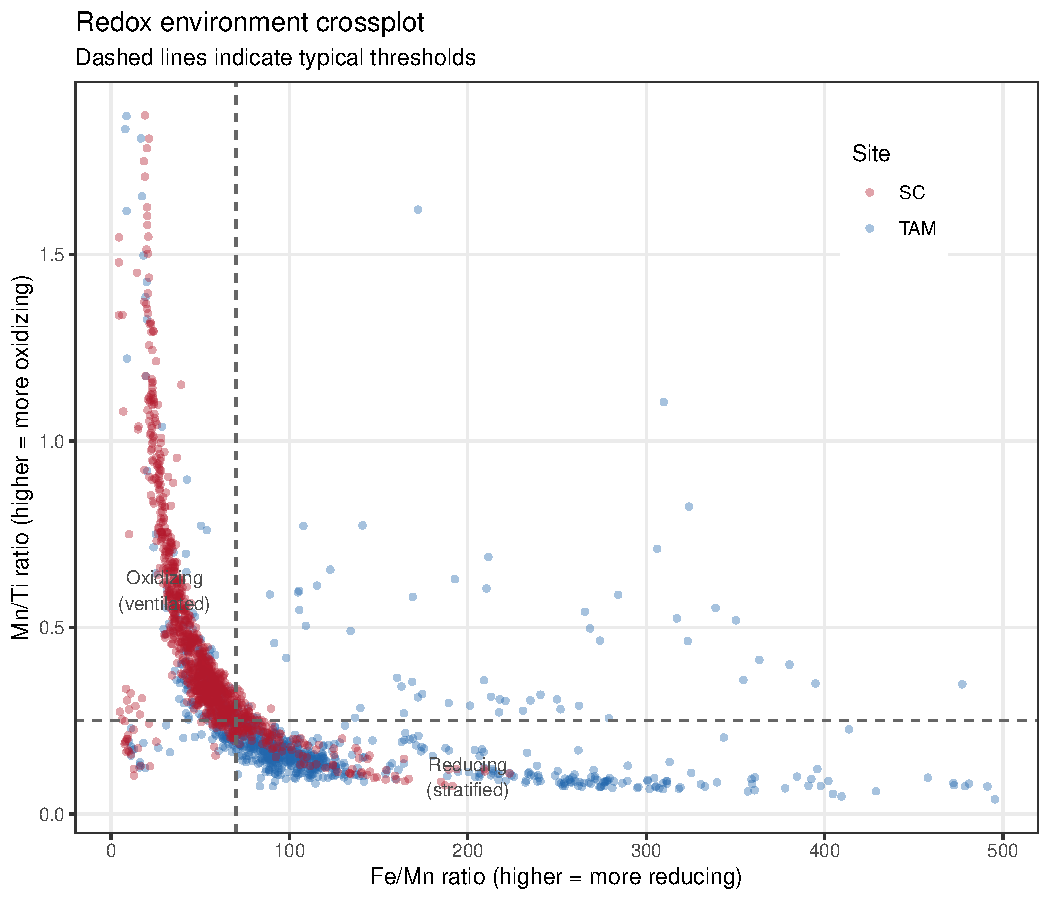
\includegraphics[width=0.8\textwidth]{figures/environmental_analysis/fig4_redox_crossplot.pdf}
\caption{Redox environment crossplot showing the inverse relationship between Fe/Mn (reducing conditions) and Mn/Ti (oxidizing conditions). TAM samples (blue) cluster in the reducing field with high Fe/Mn and low Mn/Ti, while SC samples (red) show more variable, generally more oxidizing conditions. Dashed lines indicate typical environmental thresholds.}
\label{fig:redox_crossplot}
\end{figure}

\subsubsection{Tamshiyacu (TAM) Environment}

TAM sediments consistently plot in the \textbf{reducing field} (high Fe/Mn, low Mn/Ti), indicating:
\begin{itemize}
\item Oxygen-depleted bottom waters
\item Possible water column stratification
\item Limited ventilation or mixing
\item More distal or restricted lake position
\end{itemize}

The median Fe/Mn of 95.1 exceeds the reducing threshold (70) in 96\% of measurements, indicating persistent anoxic or dysoxic conditions.

\subsubsection{Santa Corina (SC) Environment}

SC sediments show more variable redox conditions with a shift toward the \textbf{oxidizing field}:
\begin{itemize}
\item Higher bottom-water oxygen levels
\item Enhanced Mn precipitation ($3.5\times$ higher than TAM)
\item Better-ventilated conditions
\item Proximity to oxygenated inflow or shallower water depth
\end{itemize}

The median Fe/Mn of 50.8 and Mn/Ti of 0.36 suggest periodic ventilation events punctuating generally reducing conditions.

\subsection{Integration with Pebas Formation Paleoenvironmental Framework}

Our XRF-derived paleoenvironmental interpretations can be evaluated against the extensive body of work on Pebas Formation paleoecology established by Wesselingh, Hoorn, Jaramillo, and colleagues \citep{Wesselingh2002, Wesselingh2006a, Wesselingh2006b, Hoorn2010}. The Tamshiyacu (TAM) locality corresponds to the well-documented IQ26 site, which exposes approximately 10~m of Middle Miocene sediments spanning Mollusc Zones MZ7--MZ8 (approximately 12~Ma).

\subsubsection{Biostratigraphic Context}

The Pebas Formation mollusc biozonation comprises twelve zones (MZ1--MZ12) spanning approximately 17--9~Ma \citep{Wesselingh2006b}. Maximum molluscan diversity occurred during MZ8, with approximately 95 species including 78 endemics. The TAM cores sample this peak-diversity interval, providing exceptional opportunity to compare geochemical and paleontological environmental indicators.

The mollusc fauna is taxonomically dominated by two families: Cochliopidae (gastropods; 86 species, 54\%) and Corbulidae (bivalves; 23 species, 15\%). Among the corbulids, the endemic Pachydontinae radiation produced 19 species across five genera, with \textit{Pachydon obliquus} being the most abundant species in the Pebas system \citep{Wesselingh2006a}.

\subsubsection{Independent Evidence for Dysoxic Conditions}

Our finding of persistently reducing conditions at TAM (median Fe/Mn = 95.1; median Mn/Ti = 0.18) is strongly supported by paleontological evidence:

\begin{enumerate}
\item \textbf{Pachydon obliquus dominance in organic-rich clays:} \citet{Wesselingh2006a} noted that \textit{P. obliquus} ``dominates the faunas of dysoxic, organic-rich, clayish intervals.'' The species' tolerance for low-oxygen conditions explains its numerical dominance precisely in the facies where we record the lowest Mn/Ti values. The thick, convex shells of pachydontine corbulids likely represent adaptation to chemical stress and common dysoxia \citep{Wesselingh2006a}.

\item \textbf{Blue smectitic clay lithology:} The Pebas Formation is characterized by ``grey or blue clays'' with high smectite content \citep{Wesselingh2002, Hoorn2010}. Blue-grey coloration in fine-grained sediments indicates reducing conditions during and after deposition, consistent with our geochemical data showing Fe retention (reduced Fe$^{2+}$) and Mn loss (reduced Mn$^{2+}$ diffusing out of sediments).

\item \textbf{Lignite-capped parasequences:} The IQ26 section consists of coarsening-upward parasequences capped by lignites \citep{Wesselingh2002}. Lignite accumulation requires waterlogged, anoxic conditions to prevent organic matter oxidation---the same conditions that produce high Fe/Mn ratios in our XRF data.
\end{enumerate}

\subsubsection{Bivalve Shell Geochemistry: Independent Proxy Validation}

Stable isotope profiles from Pebas Formation bivalves provide independent constraints on depositional conditions \citep{Kaandorp2005}:

\begin{description}
\item[Lacustrine group (Pachydontinae):] Characterized by ``very low amplitude and irregular isotope signals,'' indicating stable, poorly-mixed water conditions consistent with stratified, dysoxic bottom waters. Our low and stable Mn/Ti values at TAM support this interpretation.

\item[Fluvial group (Unionoidea: \textit{Diplodon}, \textit{Anodontites}):] Show ``regular, high-amplitude cyclicity in both $\delta^{13}$C and $\delta^{18}$O,'' reflecting seasonal variation in well-mixed, oxygenated waters. The higher Mn/Ti variability at SC (CV = 0.81) may reflect similar periodic oxygenation events.
\end{description}

The Sr isotope composition of Pebas molluscs identifies Andean runoff as the dominant water source, with occasional cratonic water input \citep{Kaandorp2005}. This external hydrological variability likely drove the oxygenation events we detect as Mn/Ti peaks, particularly at the more fluvially-influenced SC locality.

\subsubsection{Carbonate Events and Shell-Rich Horizons}

Our highest Ca/Ti values (e.g., SC-5-6-7ABC-B at 704~mm with Ca/Ti = 48.4; TAM-1-2-3B-B at 1204--1213~mm with Ca/Ti = 34--42) likely correspond to shell-rich horizons or ``coquinas'' well-documented in the Pebas Formation. \citet{Wesselingh2002} described mollusk shell beds as characteristic facies, often representing transgressive lags or storm deposits.

The decoupling of Ca/Ti and Mn/Ti at some intervals (high carbonate under reducing conditions) may reflect:
\begin{itemize}
\item Transport of shells from shallower, oxic habitats into deeper dysoxic zones
\item Authigenic carbonate precipitation in anoxic porewaters
\item Time-averaging of shells accumulated during brief oxygenation events
\end{itemize}

\subsubsection{Site Differences in Regional Context}

The geochemical contrast between TAM and SC mirrors the environmental heterogeneity documented across the Pebas mega-wetland:

\begin{description}
\item[TAM (reducing, carbonate-rich):] Represents the ``shallow lacustrine'' to ``lacustrine'' environments described by \citet{Wesselingh2002}, with persistent water column stratification, dysoxic bottom waters, and pachydontine-dominated faunas. The 3.3$\times$ higher Ca/Ti at TAM (median 5.04 vs 2.94) reflects enhanced carbonate preservation under reducing conditions and/or proximity to productive shell-accumulating environments.

\item[SC (periodically oxic, detrital-rich):] Represents more ``fluvio-lacustrine'' conditions with better bottom-water ventilation, higher siliciclastic input (50\% more Ti), and enhanced Mn cycling. The 2$\times$ higher Mn/Ti at SC (median 0.37 vs 0.18) indicates more frequent or sustained oxygenation events, consistent with proximity to fluvial input bringing oxygenated Andean runoff.
\end{description}

\subsection{Environmental Synthesis}

The geochemical data support a model where TAM and SC represent distinct depositional environments within the Pebas mega-wetland system:

\begin{description}
\item[TAM:] More \textbf{restricted lacustrine setting} with persistent water column stratification, reduced bottom-water oxygen, elevated carbonate production or preservation, and lower siliciclastic dilution. This environment may represent a more distal position within the lake system or a protected embayment with limited circulation.

\item[SC:] More \textbf{dynamic fluvially-influenced setting} with better bottom-water ventilation, higher detrital input (50\% more Ti), enhanced Mn cycling, and more variable environmental conditions. This environment suggests proximity to fluvial sources or a more open-water position subject to periodic mixing.
\end{description}

The preserved geochemical variability within sections (particularly TAM-1-2-3B-A) indicates that environmental conditions fluctuated substantially through time, as recorded in the stratigraphic succession from older (deeper) to younger (shallower) sediments. Individual core sections span timescales estimated at $10^2$--$10^4$ years based on typical Pebas Formation sedimentation rates. These temporal fluctuations likely reflect climate-driven changes in lake level, productivity, and/or runoff intensity.

\subsection{Key Intervals for Presentation}

For paleoenvironmental presentations highlighting the Pebas Formation's dynamic environmental history, we recommend the following intervals based on signal strength and interpretive clarity (Table~\ref{tab:presentation_intervals}).

\begin{table}[htbp]
\centering
\caption{Recommended core intervals for presentation, ranked by signal clarity and paleoenvironmental significance.}
\label{tab:presentation_intervals}
\small
\begin{tabular}{llcp{5.5cm}}
\toprule
Section & Depth (mm) & Signal Type & Paleoenvironmental Interpretation \\
\midrule
\multicolumn{4}{l}{\textit{Dramatic Redox Transitions}} \\
SC-1ABC-2-3C-A-RUN1 & 367 & Mn/Ti +833\% & Most extreme oxygenation event \\
TAM-5AB-6-7-B-RUN2 & 648 & Mn/Ti +482\% & Abrupt ventilation event \\
SC-1ABC-2-3C-A-RUN1 & 184 & Mn/Ti +337\% & Second major oxygenation pulse \\
\midrule
\multicolumn{4}{l}{\textit{Concordant Oxic-Carbonate Events (Independent Proxies)}} \\
SC-3AB-4ABCD-RUN2-F & 1254--1260 & Mn/Ti + Ca/Ti & Textbook oxygenation-productivity coupling \\
SC-5-6-7ABC-C & 848 & Mn/Ti + Ca/Ti & Clear concordant event \\
TAM-5AB-6-7-B-RUN2 & 264--285 & Mn/Ti + Ca/Ti & Sustained favorable conditions \\
TAM-1-2-3B-A & 519--522 & Mn/Ti + Ca/Ti & Strongest TAM concordant interval \\
\midrule
\multicolumn{4}{l}{\textit{Extreme Carbonate Events}} \\
SC-5-6-7ABC-B & 704 & Ca/Ti = 48 & Highest carbonate; shell-rich horizon \\
TAM-1-2-3B-B & 1204--1213 & Ca/Ti = 34--42 & Major TAM carbonate pulse \\
\midrule
\multicolumn{4}{l}{\textit{Site Contrast Demonstrations}} \\
TAM-1-2-3B-A & Full section & High variability & Most dynamic TAM section (CV = 1.28) \\
SC-5-6-7ABC-B & Full section & High variability & Best SC section; widest Mn/Ti range \\
\bottomrule
\end{tabular}
\end{table}

\subsubsection{Presentation Strategy}

For maximum visual impact in presentations:

\begin{enumerate}
\item \textbf{Site contrast:} Display TAM-1-2-3B-A alongside SC-5-6-7ABC-B to illustrate the fundamental environmental difference between reducing (TAM) and periodically oxic (SC) settings. The 2-fold difference in median Mn/Ti (0.18 vs 0.37) is immediately apparent.

\item \textbf{Dramatic transitions:} The SC-1ABC-2-3C-A-RUN1 section at 367~mm shows an 833\% Mn/Ti increase---the most extreme single-point transition in the dataset. This visually demonstrates the rapidity of environmental change in the Pebas system.

\item \textbf{Independent proxy concordance:} The SC-3AB-4ABCD-RUN2-F interval at 1254--1260~mm shows simultaneous Mn/Ti and Ca/Ti peaks, demonstrating genuine multi-proxy evidence for oxic, productive conditions without the spurious correlation concerns of Fe/Mn--Mn/Ti comparisons.

\item \textbf{Carbonate events:} The SC-5-6-7ABC-B shell horizon at 704~mm (Ca/Ti = 48.4) provides a striking visual anchor for discussing shell-rich facies and their paleoenvironmental significance.
\end{enumerate}

\subsection{Recommendations for Future Work}

Based on this analysis, we recommend:

\begin{enumerate}
\item Use \textbf{Mn/Ti as the primary redox proxy} (detrital-corrected, avoids Fe ambiguity)
\item Pair with \textbf{Ca/Ti as an independent carbonate proxy} for multi-proxy confirmation
\item Interpret \textbf{Fe/Mn as supporting evidence only}, acknowledging shared-element constraints with Mn/Ti
\item Focus detailed paleoenvironmental reconstruction on \textbf{TAM-1-2-3B-A} (extreme variability), \textbf{TAM-5AB-6-7-B-RUN2} (clear transitions), and \textbf{SC-1ABC-2-3C-A-RUN1} (dramatic events)
\item Use \textbf{SC-5-6-7ABC-B} as the representative SC comparison section (highest $n$, widest dynamic range)
\item Avoid sections with $<30$ measurements or $<100$ mm stratigraphic coverage
\item Consider log-ratio transformations (centered log-ratio or isometric log-ratio) for formal statistical analysis of compositional data
\end{enumerate}
